\begin{frame}[allowframebreaks]
\frametitle{Arquitectura UNet}
    \begin{figure}
        \centering
        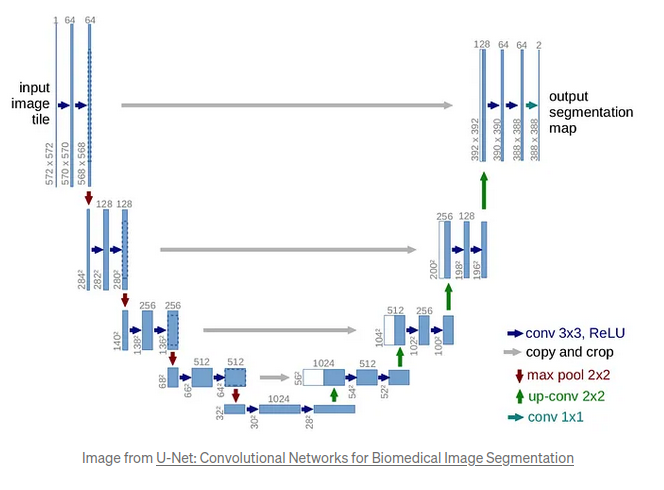
\includegraphics[scale=0.3]{img/section_07/UNet.png}
        \caption{Esquema base}
        \label{fig:unet-base}
    \end{figure}

    \begin{figure}
        \centering
        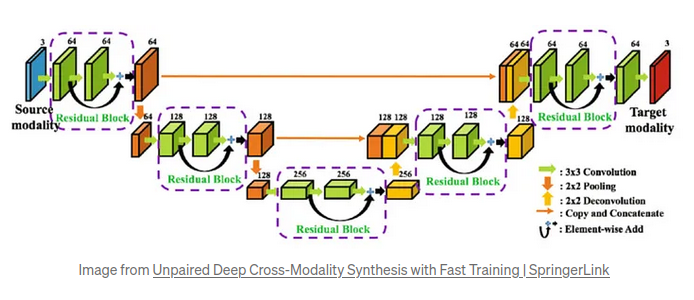
\includegraphics[scale=0.3]{img/section_07/ResUNet.png}
        \caption{Conexiones residuales}
        \label{fig:res-unet}
    \end{figure}

    \begin{figure}
        \centering
        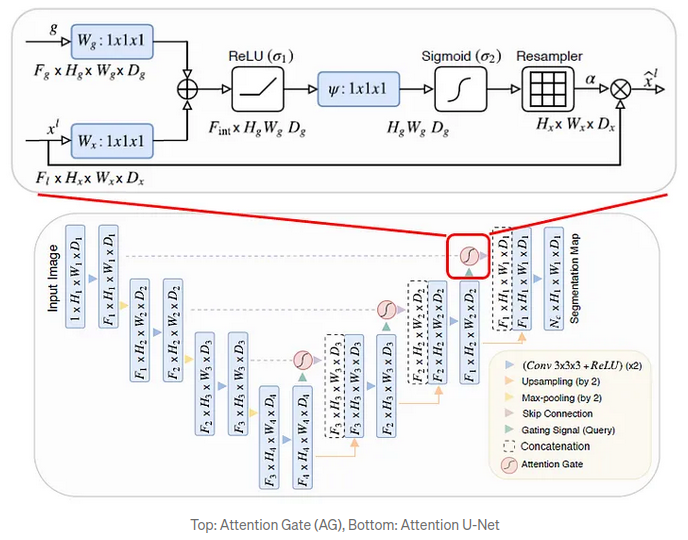
\includegraphics[scale=0.3]{img/section_07/Attention_UNet.png}
        \caption{Atención}
        \label{fig:attn-unet}
    \end{figure}

    \begin{figure}
        \centering
        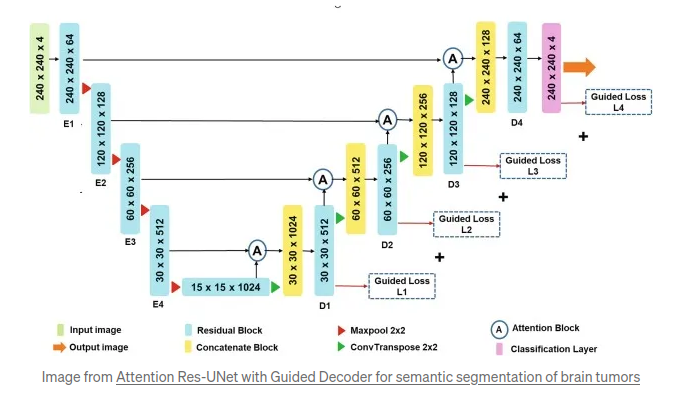
\includegraphics[scale=0.3]{img/section_07/Attention_ResUNet.png}
        \caption{Atención + Conexiones residuales}
        \label{fig:att-res-unet}
    \end{figure}
\end{frame}

\begin{frame}{Transformada Wavelet}
    Las wavelets son señales, o formas de onda, las cuales tienen una duración limitada y un valor promedio de cero. Las wavelets pueden ser irregulares y asimétricas, características que les otorgan una mejor adaptación en el análisis de señales en comparación con la transformada de Fourier.

    \begin{figure}
        \centering
        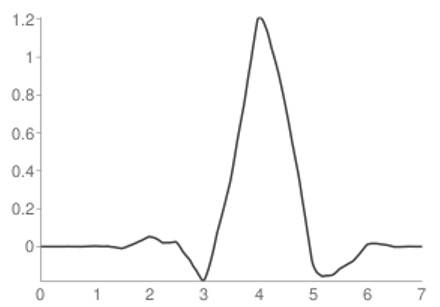
\includegraphics[scale=0.3]{img/section_07/Symlet-4.jpg}
        \caption{Symlet 4}
        \label{fig:symlet4}
    \end{figure}
\end{frame}

\begin{frame}
    De forma general la transformada wavelet descompone una señal mediante el uso de las versiones escaladas y desplazadas de la wavelet madre.

    \begin{figure}
        \centering
        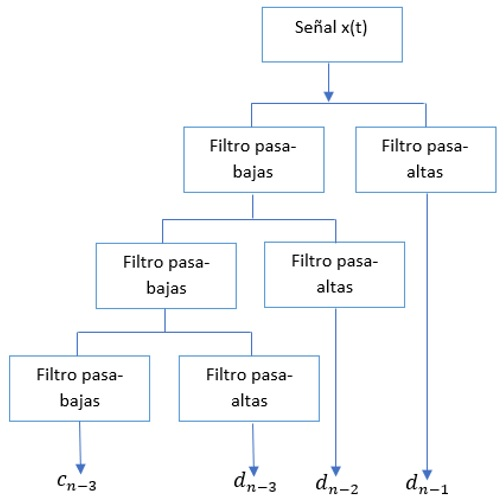
\includegraphics[scale=0.3]{img/section_07/Filtros.jpg}
        \caption{Filtros}
        \label{fig:filtros}
    \end{figure}
\end{frame}

\begin{frame}{Descomposición por Wavelets}
    \begin{figure}
        \centering
        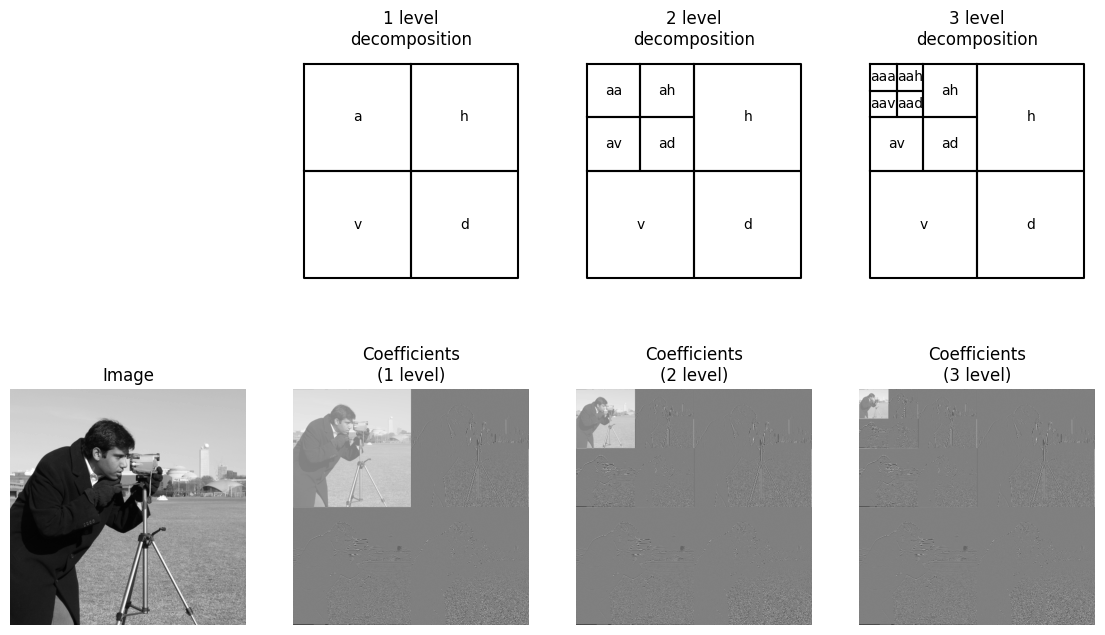
\includegraphics[scale=0.4]{img/section_07/Wavelets_decomposition.png}
        \caption{Descomposición por Wavelets}
        \label{fig:descomposicion}
    \end{figure}
\end{frame}

\begin{frame}{Retos}
    \begin{figure}
    \centering
    \begin{tabular}{cc}
         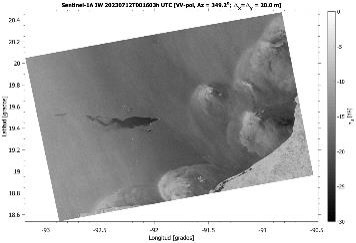
\includegraphics[scale=0.45]{img/section_07/derrame.jpg} &
         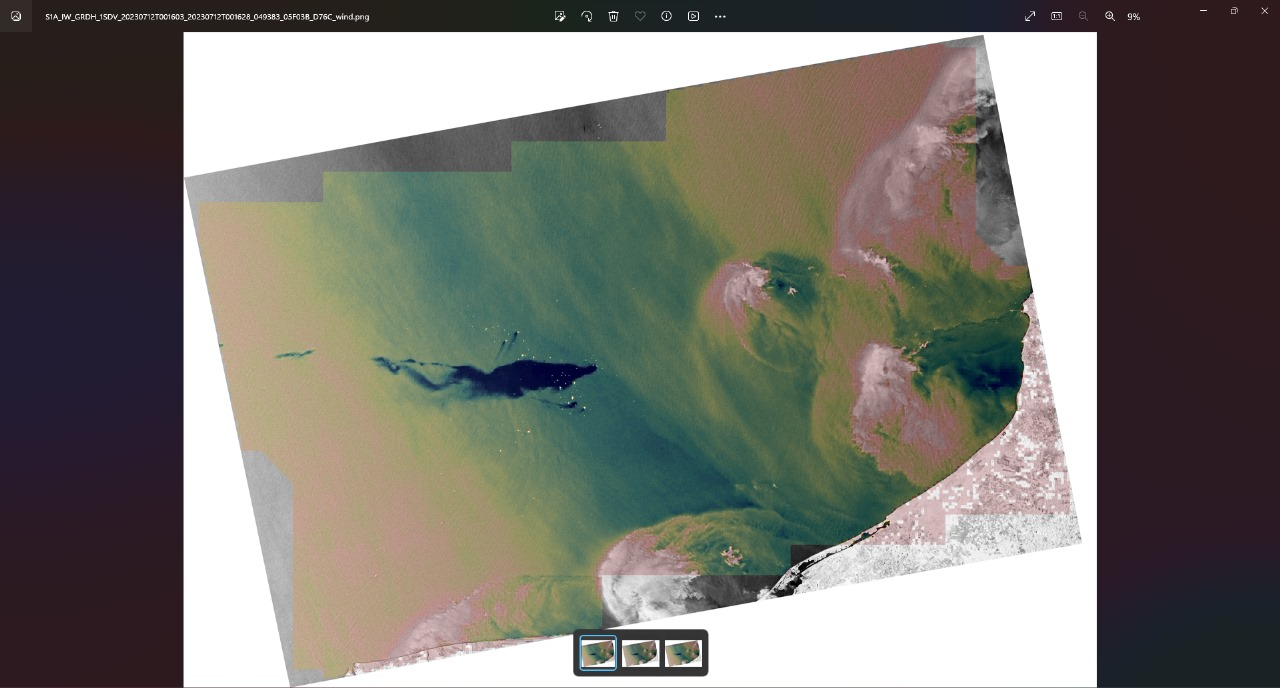
\includegraphics[scale=0.15]{img/section_07/campo_viento.jpg}\\
         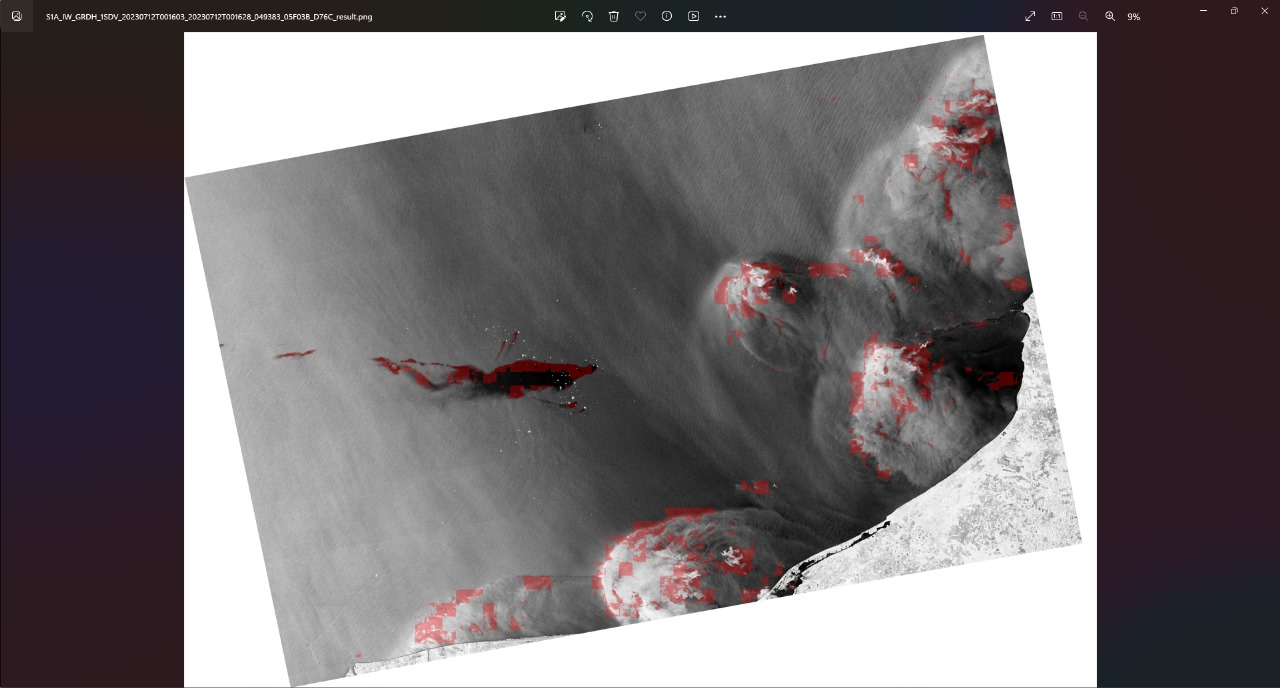
\includegraphics[scale=0.15]{img/section_07/segmentacion_01.jpg}& 
         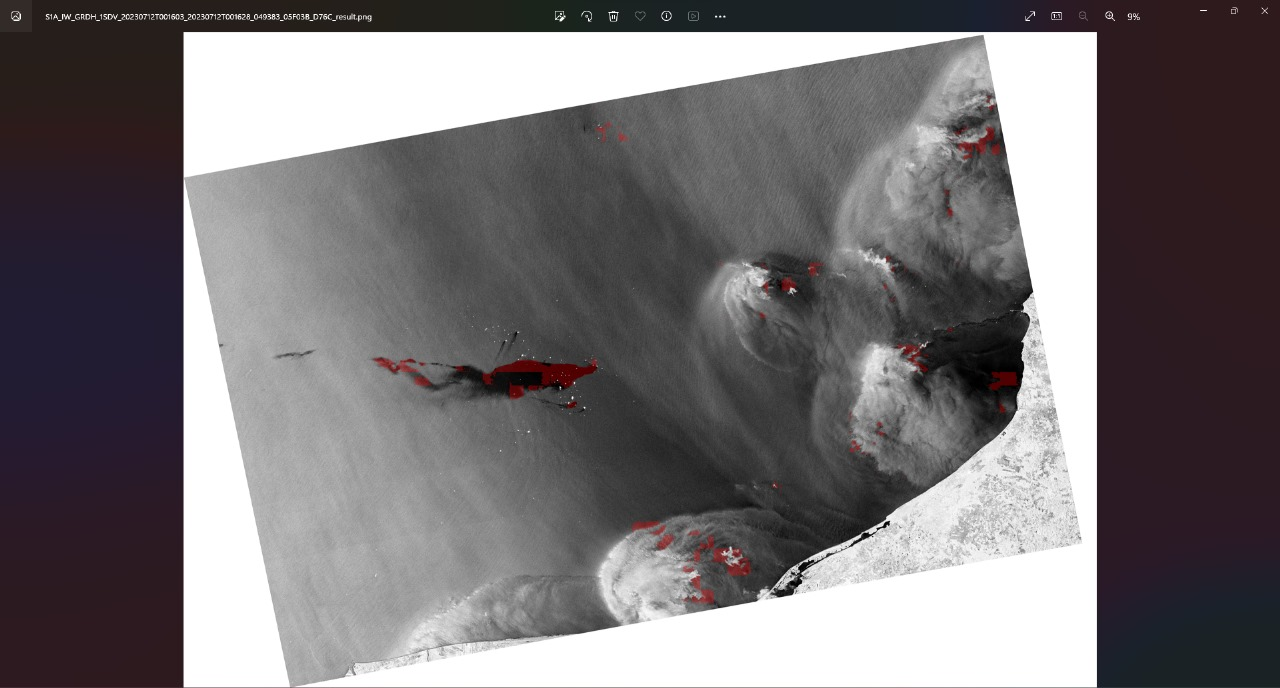
\includegraphics[scale=0.15]{img/section_07/segmentacion_02.jpg}
    \end{tabular}
    \caption{Resultado de la segmentación en Sentinel 1}
    \label{fig:my_label}
\end{figure}
\end{frame}

\begin{frame}{Retos}
    \begin{figure}
        \centering
        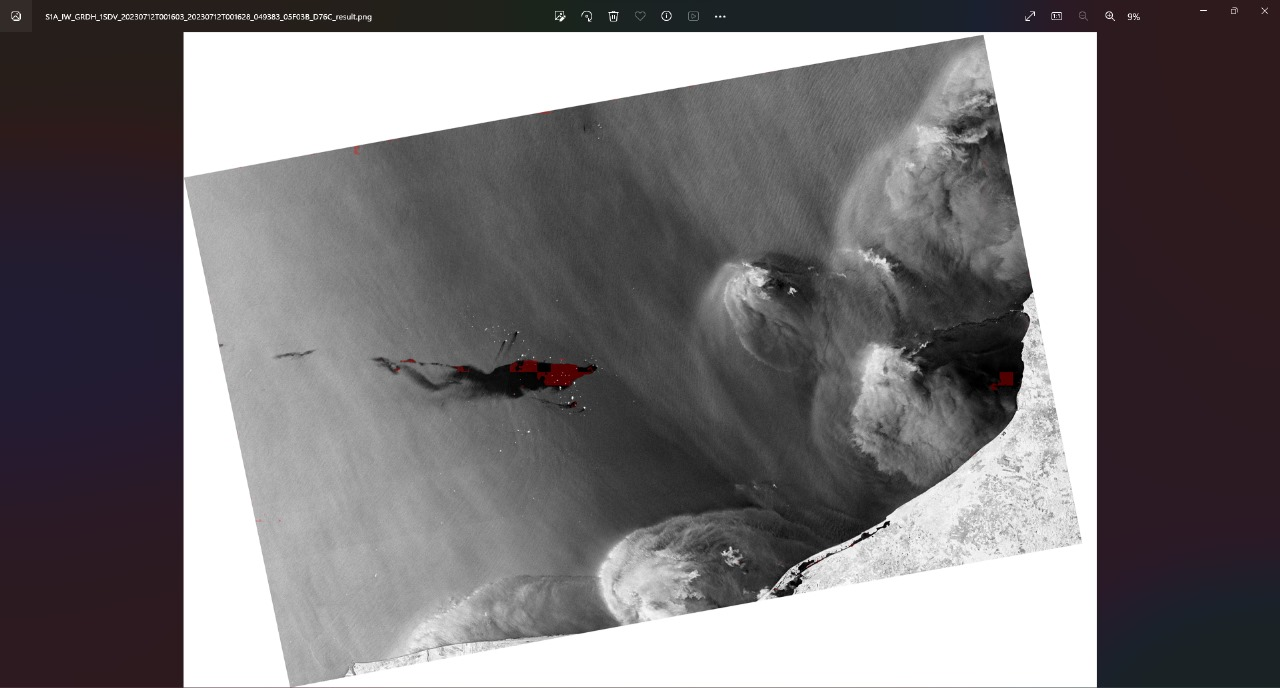
\includegraphics[scale=0.3]{img/section_07/segmentacion_03.jpg}
        \caption{Falsos positivos}
        \label{fig:enter-label}
    \end{figure}
\end{frame}

\begin{frame}{Retos}
    \begin{itemize}
        \item Ampliación del dataset.- el entrenamiento se ha realizado con un conjunto de imágenes Envisat.
        
        \item Entrenamiento distribuido.- cada iteración con el dataset (~80,000 imágenes) tarda aproximadamente entre 30 y 40 minutos.
        
        \item Integración de canales adicionales.- bandas multiespectrales e hiperespectrales.        
        \item Integración de otros marcos de descomposición (ridgelets, curvlets, shearlets)
    \end{itemize}
\end{frame}
